\documentclass[11pt,psfig]{article}
\usepackage{epsfig}
\usepackage{times}
\usepackage{amssymb}
\usepackage{float}

\newcount\refno\refno=1
\def\ref{\the\refno \global\advance\refno by 1}
\def\ux{\underline{x}}
\def\uw{\underline{w}}
\def\bw{\underline{w}}
\def\ut{\underline{\theta}}
\def\umu{\underline{\mu}} 
\def\bmu{\underline{\mu}} 
\def\be{p_e^*}
\newcount\eqnumber\eqnumber=1
\def\eq{\the \eqnumber \global\advance\eqnumber by 1}
\def\eqs{\eq}
\def\eqn{\eqno(\eq)}

 \pagestyle{empty}
\def\baselinestretch{1.1}
\topmargin1in \headsep0.3in
\topmargin0in \oddsidemargin0in \textwidth6.5in \textheight8.5in
\begin{document}
\setlength{\parskip}{1.2ex plus0.3ex minus 0.3ex}


\thispagestyle{empty} \pagestyle{myheadings} \markright{Homework
3: CS 216, Image Understanding: Spring 2014}



\title{CS 216 Homework \#}
\author{Zachary DeStefano, 15247592}
\date{Due Date: May 9, 2014 in class}

\maketitle

\vfill\eject

\newpage

\section*{Problem 1}

\subsection*{k-Means Clustering results}

\begin{figure}[H]
\centering
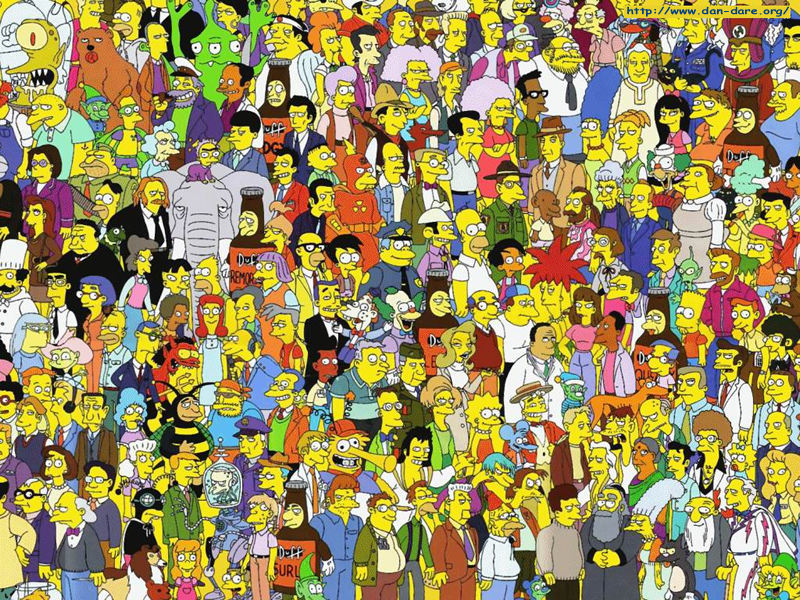
\includegraphics[height=3in]{simpsons.jpg}
\caption{Original Image}
\end{figure}

\begin{figure}[H]
\centering
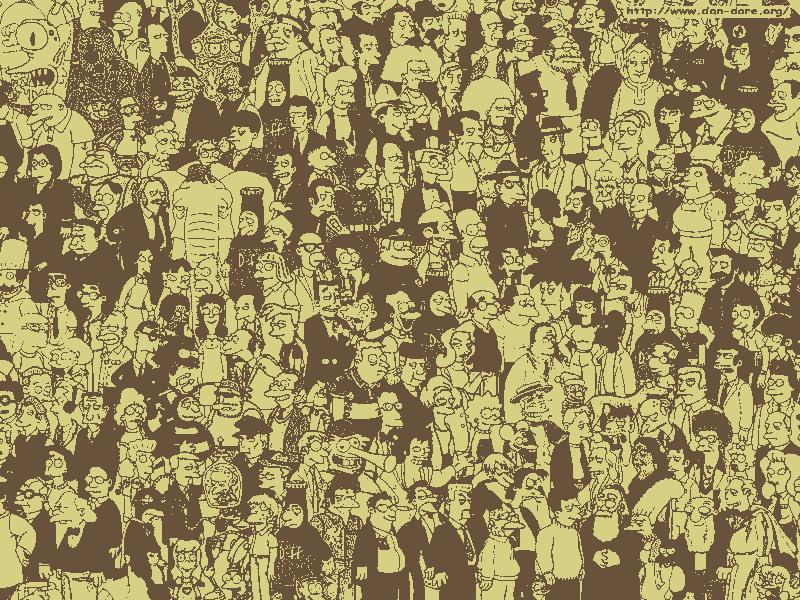
\includegraphics[height=3in]{2-means_simpsons.jpg}
\caption{The k-Means Image when $k=2$}
\end{figure}

\begin{figure}[H]
\centering
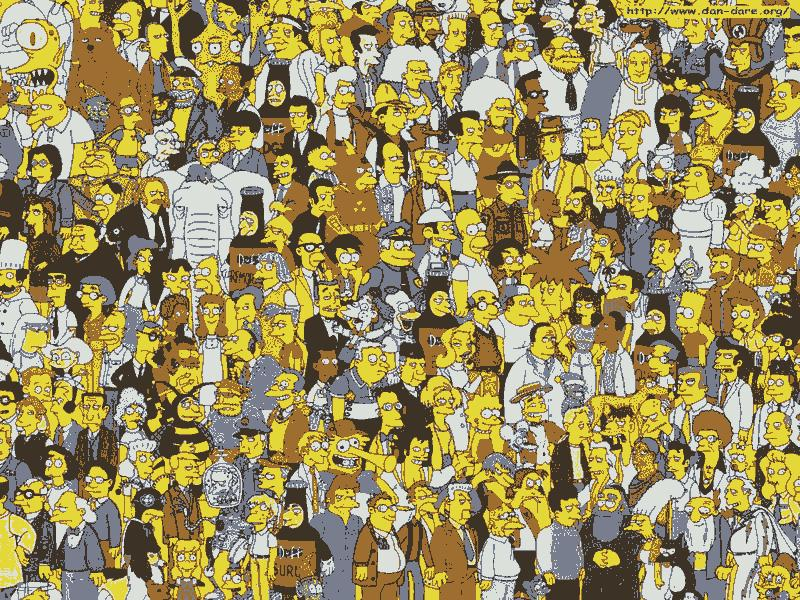
\includegraphics[height=3in]{5-means_simpsons.jpg}
\caption{The k-Means Image when $k=5$}
\end{figure}

\begin{figure}[H]
\centering
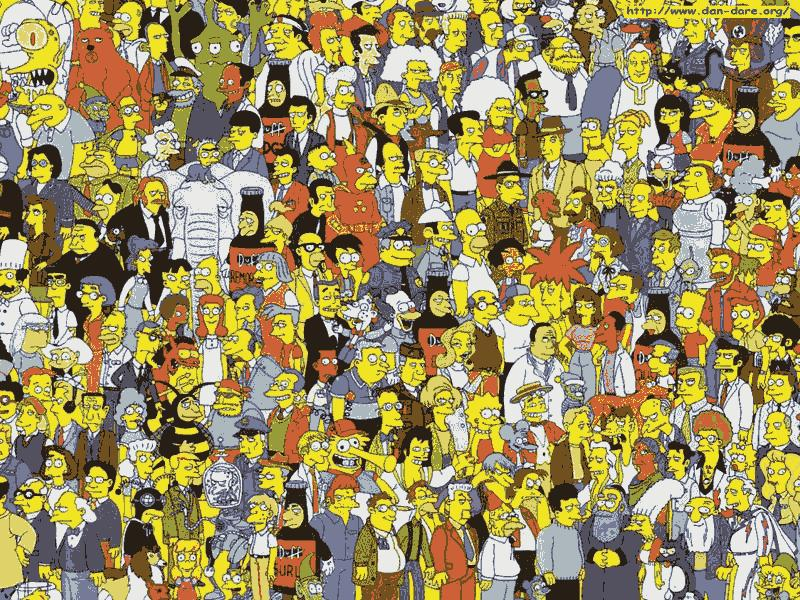
\includegraphics[height=3in]{10-means_simpsons.jpg}
\caption{The k-Means Image when $k=10$}
\end{figure}

\subsection*{Result when skewing the Red Channel}

If we multiply the red channel by 100, then the mean will tend more toward the red channel than the other channels. The result will be a red tint on the final result image. That is exactly what happened with the following images which are the same k-means images as above but the red channel was multiplied by 100 before k-Means was done. 

\begin{figure}[H]
\centering
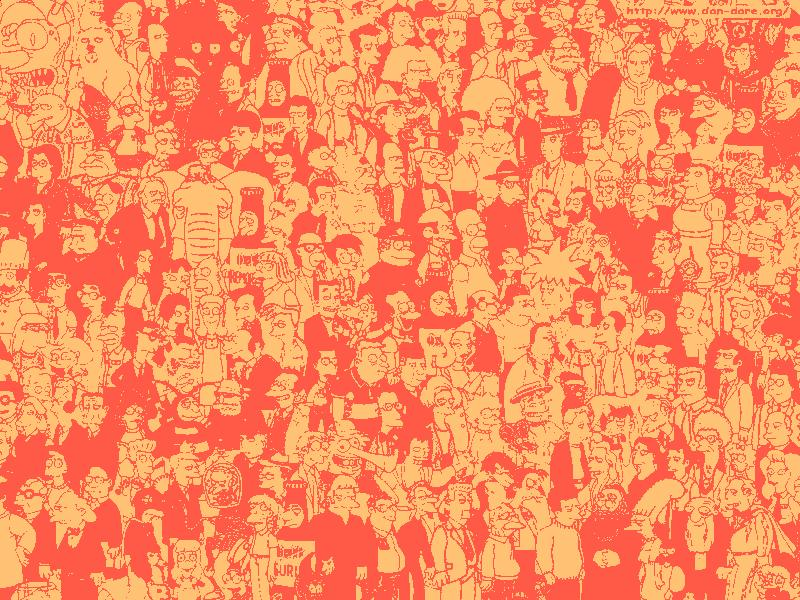
\includegraphics[height=3in]{2-means_redEn_simpsons.jpg}
\caption{The k-Means Image when $k=2$ and a skewed red channel}
\end{figure}

\begin{figure}[H]
\centering
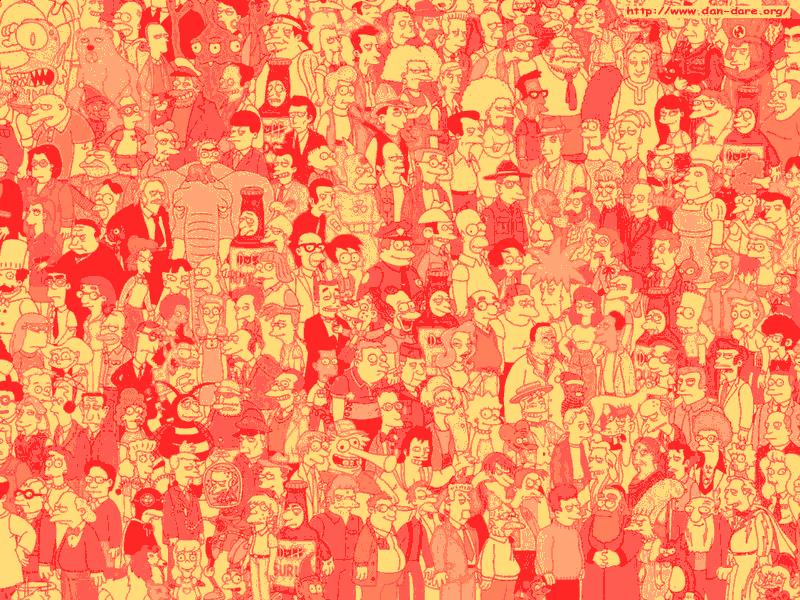
\includegraphics[height=3in]{5-means_redEn_simpsons.jpg}
\caption{The k-Means Image when $k=5$ and a skewed red channel}
\end{figure}

\begin{figure}[H]
\centering
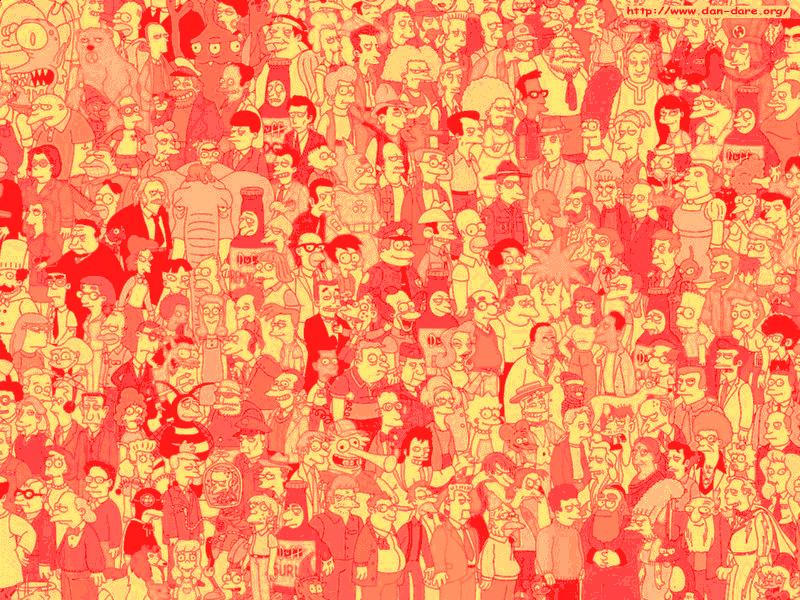
\includegraphics[height=3in]{10-means_redEn_simpsons.jpg}
\caption{The k-Means Image when $k=10$ and a skewed red channel}
\end{figure}

\end{document}








